\documentclass[tikz,border=5pt]{standalone}
\usepackage[T1]{fontenc}
\usepackage{lmodern,amsmath,amssymb}
\usetikzlibrary{arrows.meta,calc,positioning,fit,backgrounds,shapes.geometric,matrix,decorations.pathreplacing,patterns}
\definecolor{ink}{gray}{0.08}
\definecolor{wash}{gray}{0.965}
\definecolor{soft}{gray}{0.45}
\tikzset{box/.style={draw=ink,line width=.65pt,fill=white,align=center,inner sep=4pt,outer sep=0pt,font=\small},flow/.style={draw=ink,line width=.65pt,-{Latex[length=1.8mm,width=1.3mm]},rounded corners=2pt},annotation/.style={font=\scriptsize,text=soft,align=center},groupbox/.style={draw=soft,dashed,line width=.45pt,fill=wash}}
\begin{document}
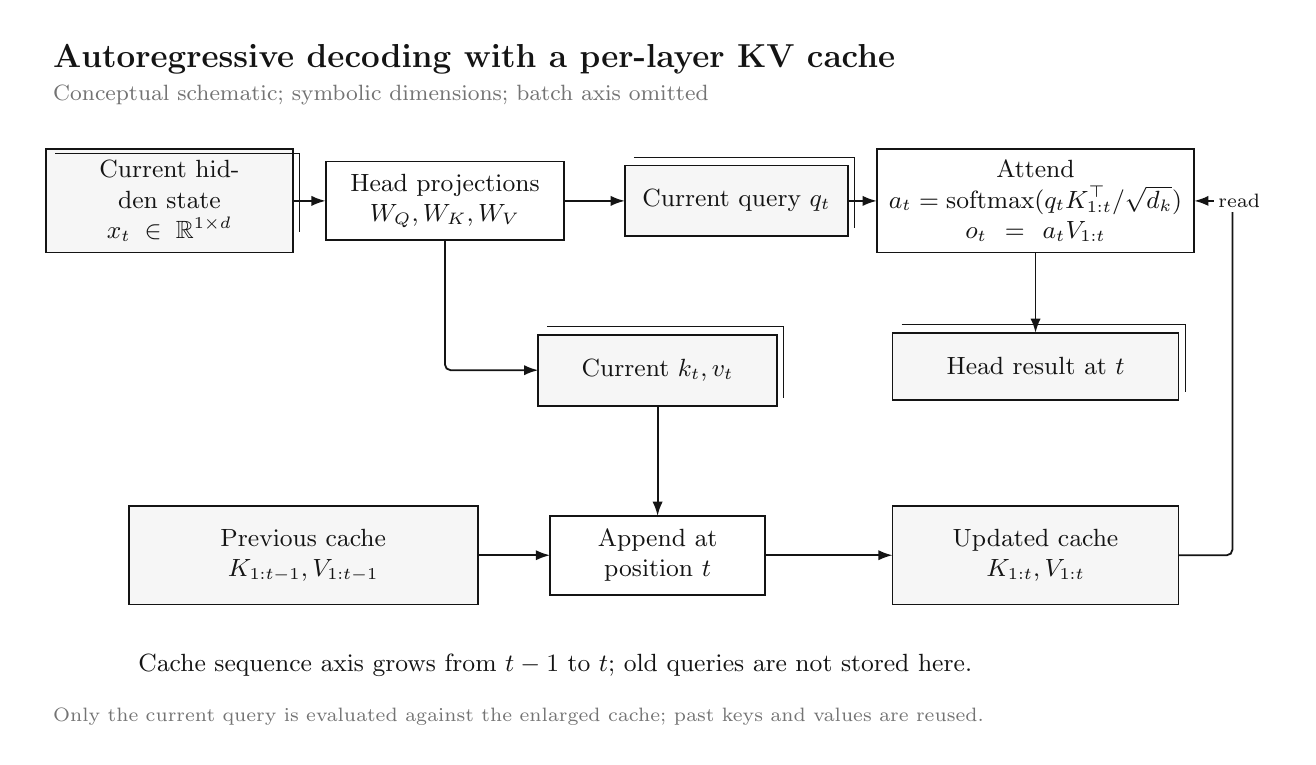
\begin{tikzpicture}[x=1cm,y=-1cm,font=\rmfamily,text=ink]

\path[use as bounding box] (0,0) rectangle (16,9);
\node[anchor=west,font=\large\bfseries] at (.2,.4) {Autoregressive decoding with a per-layer KV cache};
\node[anchor=west,font=\footnotesize,text=soft] at (.2,.85) {Conceptual schematic; symbolic dimensions; batch axis omitted};
\begin{pgfonlayer}{background}
\end{pgfonlayer}
\node[box,fill=wash,minimum width=3.1cm,minimum height=1.0cm,text width=2.85cm] (x) at (1.8,2.2) {Current hidden state\\$x_t\in\mathbb{R}^{1\times d}$};
\draw[ink,line width=.4pt] (0.35,1.6) -- (3.45,1.6) -- (3.45,2.6);
\node[box,minimum width=3.0cm,minimum height=1.0cm,text width=2.75cm] (proj) at (5.3,2.2) {Head projections\\$W_Q,W_K,W_V$};
\node[box,fill=wash,minimum width=2.8cm,minimum height=0.9cm,text width=2.55cm] (q) at (9,2.2) {Current query $q_t$};
\draw[ink,line width=.4pt] (7.699999999999999,1.6500000000000001) -- (10.5,1.6500000000000001) -- (10.5,2.5500000000000003);
\node[box,minimum width=4.0cm,minimum height=1.3cm,text width=3.75cm] (attn) at (12.8,2.2) {Attend\\$a_t=\operatorname{softmax}(q_t K_{1:t}^{\top}/\sqrt{d_k})$\\$o_t=a_tV_{1:t}$};
\node[box,fill=wash,minimum width=3cm,minimum height=0.9cm,text width=2.75cm] (new) at (8,4.35) {Current $k_t,v_t$};
\draw[ink,line width=.4pt] (6.6,3.7999999999999994) -- (9.6,3.7999999999999994) -- (9.6,4.7);
\node[box,fill=wash,minimum width=4.4cm,minimum height=1.25cm,text width=4.15cm] (old) at (3.5,6.7) {Previous cache\\$K_{1:t-1},V_{1:t-1}$};
\node[box,minimum width=2.7cm,minimum height=1.0cm,text width=2.45cm] (append) at (8,6.7) {Append at\\position $t$};
\node[box,fill=wash,minimum width=3.6cm,minimum height=1.25cm,text width=3.35cm] (cache) at (12.8,6.7) {Updated cache\\$K_{1:t},V_{1:t}$};
\node[box,fill=wash,minimum width=3.6cm,minimum height=0.85cm,text width=3.35cm] (out) at (12.8,4.3) {Head result at $t$};
\draw[ink,line width=.4pt] (11.1,3.775) -- (14.700000000000001,3.775) -- (14.700000000000001,4.625);
\node[align=center,inner sep=0pt,outer sep=0pt,font=\small,minimum width=11cm,minimum height=0.5cm,text width=10.75cm] (note9) at (6.7,8.1) {Cache sequence axis grows from $t-1$ to $t$; old queries are not stored here.};
\begin{pgfonlayer}{background}
\draw[flow] (x.east) -- (proj.west);
\draw[flow] (proj.east) -- (q.west);
\draw[flow] (q.east) -- (attn.west);
\draw[flow] (attn.south) -- (out.north);
\draw[flow] (proj.south) -- (5.3,4.35) -- (new.west);
\draw[flow] (new.south) -- (append.north);
\draw[flow] (old.east) -- (append.west);
\draw[flow] (append.east) -- (cache.west);
\draw[flow] (cache.east) -- (15.3,6.7) -- (15.3,2.2) -- (attn.east) node[midway,right,fill=white,inner sep=1.5pt,font=\scriptsize] {read};
\end{pgfonlayer}
\node[anchor=west,align=left,font=\scriptsize,text=soft,text width=15.6cm] at (.2,8.75) {Only the current query is evaluated against the enlarged cache; past keys and values are reused.};
\end{tikzpicture}
\end{document}
